%%%%%%%%%%%%%%%%%%%%%%%%%%%%%%%%%%%%%%%%%%%%%%%%%%%%%%%
%%% 可能用到的网站`'
%%%%%%%%%%%%%%%%%%%%%%%%%%%%%%%%%%%%%%%%%%%%%%%%%%%%%%%
%%% LaTeX公式编辑器:https://www.latexlive.com/
%%% Diagram流程图绘制:https://www.drawio.com/
%%%%%%%%%%%%%%%%%%%%%%%%%%%%%%%%%%%%%%%%%%%%%%%%%%%%%%%

%%%%%%%%%%%%%%%%%%%%%%%%%%%%%%%%%%%%%%%%%%%%%%%%%%%%%%%
%%% 模板参数设置
%%%%%%%%%%%%%%%%%%%%%%%%%%%%%%%%%%%%%%%%%%%%%%%%%%%%%%%
\documentclass{mcmthesis}  % 文档类型
\mcmsetup{
        tcn = 12345678,   % 队伍控制号
        problem = ABCDEF,  % 选题
        sheet = true,   % sheet页
        titleinsheet = true,   % sheet页显示标题
        keywordsinsheet = true,  % sheet页显示关键词
        titlepage = false,   % 标题页
        abstract = true  % 摘要
        }
%%%%%%%%%%%%%%%%%%%%%%%%%%%%%%%%%%%%%%%%%%%%%%%%%%%%%%%

%%%%%%%%%%%%%%%%%%%%%%%%%%%%%%%%%%%%%%%%%%%%%%%%%%%%%%%
%%% 导入宏包和引用文献源
%%%%%%%%%%%%%%%%%%%%%%%%%%%%%%%%%%%%%%%%%%%%%%%%%%%%%%%
\usepackage{palatino}  % 帕拉提诺体字体宏包
\usepackage{lastpage}  % 引入 lastpage 宏包
\usepackage{lipsum}  % 导入生成段落的宏包
\usepackage[hyperref=true,style=ieee]{biblatex}  % biblatex参考文献宏包
\addbibresource{ref.bib}  % 添加引用文献bib源
\newcommand{\upcite}[1]{\textsuperscript{\cite{#1}}}
%%%%%%%%%%%%%%%%%%%%%%%%%%%%%%%%%%%%%%%%%%%%%%%%%%%%%%%

%%%%%%%%%%%%%%%%%%%%%%%%%%%%%%%%%%%%%%%%%%%%%%%%%%%%%%%
%%% 文档信息设置
%%%%%%%%%%%%%%%%%%%%%%%%%%%%%%%%%%%%%%%%%%%%%%%%%%%%%%%
\title{The MCM Thesis of Team 12345678}  % 文章标题
\author{\small Team 12345678}  % 作者,开启标题页才会显示
\date{\today}  % 日期,开启标题页才会显示

\memoto{MCM office}  % 建议书目标
\memofrom{MCM Team 12345678}  % 建议书来源
\memosubject{MCM}  % 建议书主题
\memodate{\today}  % 建议书日期
%%%%%%%%%%%%%%%%%%%%%%%%%%%%%%%%%%%%%%%%%%%%%%%%%%%%%%%

%%%%%%%%%%%%%%%%%%%%%%%%%%%%%%%%%%%%%%%%%%%%%%%%%%%%%%%
%%% 文档开始
%%%%%%%%%%%%%%%%%%%%%%%%%%%%%%%%%%%%%%%%%%%%%%%%%%%%%%%
\begin{document}  % 文档
\begin{abstract}  % 摘要
This is a summary.
\begin{keywords}  % 关键词
keyword1, keyword2, keyword3
\end{keywords}  % 结束关键词
\end{abstract}  % 结束摘要
\maketitle  % 生成sheet页

\tableofcontents  % 生成目录表

%%%%%%%%%%%%%%%%%% sheet页与目录页结束 %%%%%%%%%%%%%%%%%%

\newpage  % 开始新的一页
\section{Introduction}  % 一级标题

\subsection{Problem Background}

Wordle, developed by Jonathan Feinberg in 2008, was created 
to help students expand their vocabulary. However, due to its
simple gameplay, it quickly went viral on social media at the 
end of 2021 and was later acquired by The New York Times in 2022, 
integrating it into their online games section. It is a web-based 
game with two difficulty modes: easy and hard. It focuses on user 
experience and game logic, and there are many variations of the game, 
such as Quordle (guessing 4 words simultaneously), Octordle 
(guessing 8 words simultaneously), and Worldle (a geography version where 
players guess a country or region). The rules for the hard mode are as follows.

\begin{figure}[htbp]  % 图片
\small
\centering  % 居中
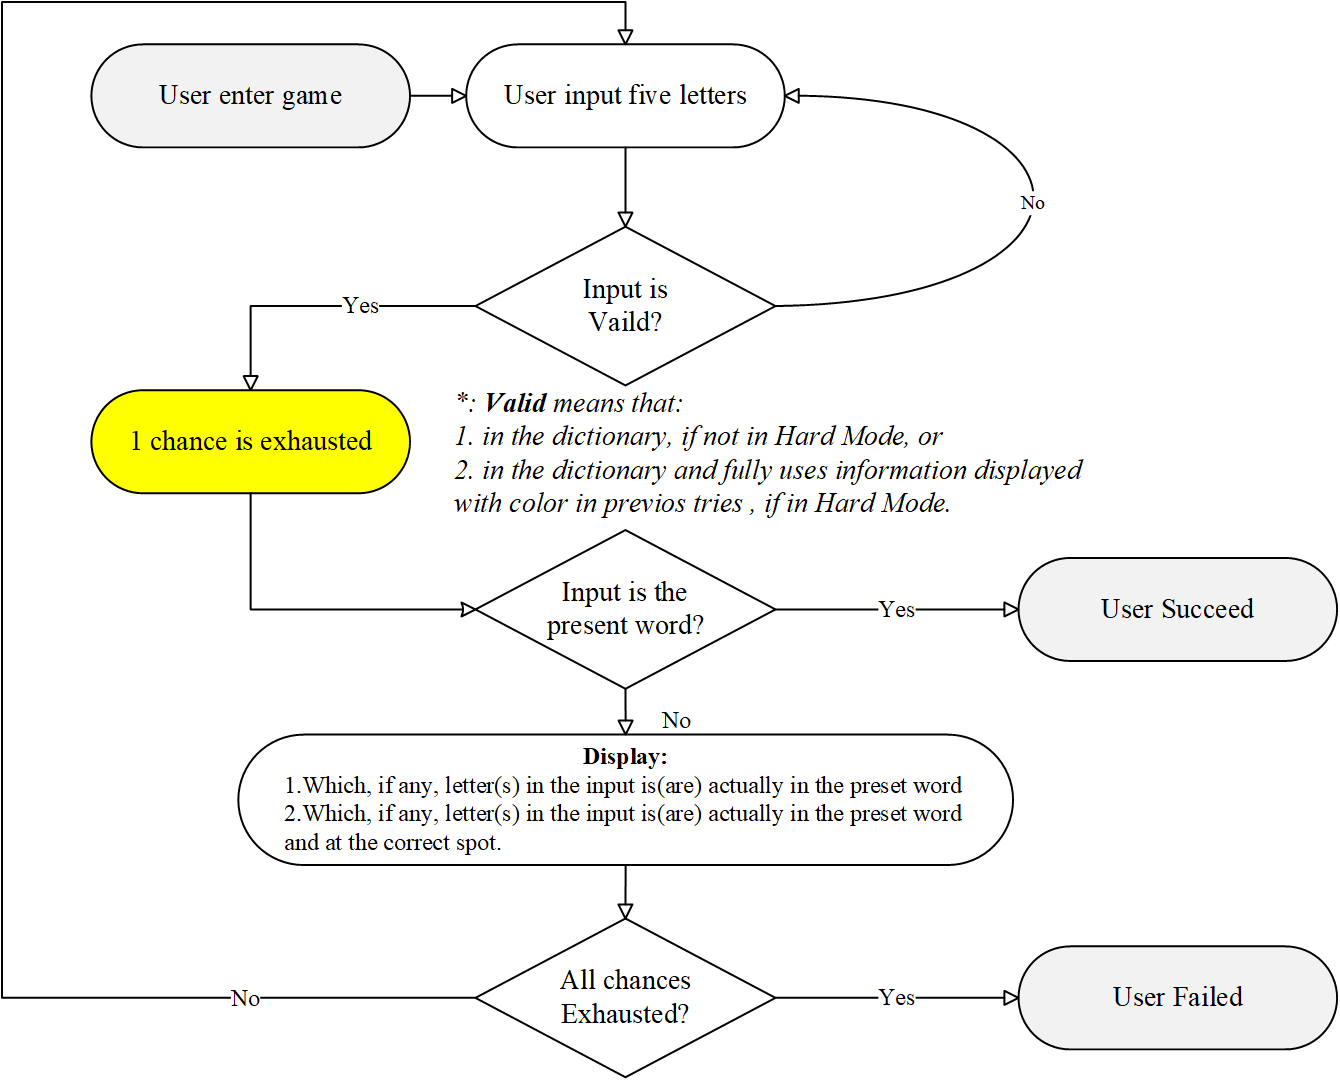
\includegraphics[width=14cm]{figure/F1.png}  % 引入图片源
\caption{Game  Rules} \label{Figure1}  % 标题与标签
\end{figure}  % 图片结束

\subsection{Restatement of the Problem}

We need to analyze the data provided by The New York Times and address the following tasks:
\begin{itemize}  % 无序列表
        \item \textbf{Problem 1: }Develop a model to explain the variations in the daily reported results and predict the 
        range of reported results for March 1, 2023. Additionally, analyze which word attributes influence 
        players' decisions to select Hard Mode.
        \item \textbf{Problem 2: }Build a prediction model to estimate the percentage distribution of results (1, 2, 3, 4, 5, 6, X) 
        for a future day, with specific predictions for "EERIE" on March 1, 2023, and assess the model's accuracy.
        \item \textbf{Problem 3: }Develop a classification model to categorize words by difficulty level and identify their attributes. 
        Conduct a detailed analysis for "EERIE" and evaluate the model's accuracy.
        \item \textbf{Problem 4: }Explore and describe any other interesting insights or patterns found within the data.
\end{itemize}  % 无序列表结束

\subsection{Our Work}

\section{Assumptions and Notations}  % 二级标题
\subsection{Assumptions}
To simplify the model, we made the following assumptions:
\begin{itemize}
        \item \textbf{Assumption 1: }The percentages provided in the data accurately reflect the actual situation with minimal falsification and can be used directly.\\
        \textbf{Justification:}Most people report their scores truthfully, as the reporting process is anonymous and has no consequences. Although some individuals 
        may choose to report false scores, the daily volume of reports is large enough that this small fraction of false data will not significantly impact the overall percentages.
        \item \textbf{Assumption 2: }The percentages of total reported scores can be used to represent the percentages of scores reported in Hard Mode.\\
        \textbf{Justification:}Due to rounding, we found that the sum of the daily reported percentages does not equal exactly 1 but still reaches 0.99, which is 
        very close to 1. Therefore, the reported percentages can effectively substitute for the actual percentages.
\end{itemize}
\subsection{Notations}
%%%%%%%%%%%%%%%%%%%%%%%% 三线表 %%%%%%%%%%%%%%%%%%%%%%%%
\begin{table}[!h]  % 表格
        \tabcolsep 84pt % 列间距
        \begin{tabular*}{\textwidth}{cccc}  % tabular*环境
        \toprule  % 顶线
        Symbol & Decription \\
        \midrule  % 中线
        $f_{t}$ & forget gate  \\
        $i_{t}$ & input gate  \\
        $o_{t}$ & output gate  \\
        $h_{t}$ & hidden state  \\
        $c_{t}$ & cell state  \\
        $x_{t}$ & LSTM's input  \\
        $W_{f,i,c,o}$ & Bias  \\
        $b_{f,i,c,o}$ & Weight Matrix \\
        $r$ & Pearson correlation\\
        \bottomrule  % 底线
        \end{tabular*}  % tabular*环境结束
\end{table}  % 表格结束
%%%%%%%%%%%%%%%%%%%%%% 三线表结束 %%%%%%%%%%%%%%%%%%%%%%
\section{Model 1-Prediction Model based on LSTM}  % 一级标题

By analyzing \textbf{$Problem\_C\_Data\_Wordle.xlsx$}, we found that the Wordle data is 
collected and analyzed daily. By analyzing this data, we can clearly 
see that the results of Wordle change over time and exhibit time dependence. 
Therefore, we chose the LSTM algorithm, which is specifically designed to 
capture and utilize long-term dependencies in sequential data. This fits 
well with the time-varying Wordle results presented in the problem. We 
ultimately used this algorithm to simulate the data for March 1, 2023.

\subsection{Description of LSTM}
LSTM is a neural network structure that can effectively capture long-term dependencies 
in time series data. By introducing gating mechanisms, it can selectively retain and 
forget information, solving the vanishing and exploding gradient problems inherent in 
raditional RNNs. Although LSTM is computationally expensive, it performs excellently in 
many tasks, especially in processing sequential data. Its main features are the memory 
cell and gating mechanisms, which introduce three gates: the forget gate, input gate, 
and output gate, allowing for selective retention or discarding of data. Its update equations 
are as follows.
\begin{equation} 
\begin{aligned}
        f_{t} &=\sigma(W_{f}\cdot [h_{t-1},x_{t}]+b_{f})\\
        i_{t} &\sigma(W_{i}\cdot [h_{t-1},x_{t}]+b_{i}) \\
        o_{t} &=\sigma(W_{o}\cdot [h_{t-1},x_{t}]+b_{o}) \\
        \tilde{c_{t}} &=tanh(W_{c}\cdot [h_{t-1},x_{t}]+b_{c})\\
        c_{t} &=f_{t}\cdot c_{t-1}+i_{t}\cdot \tilde{c_{t}} \\
        h_{t} &=o_{t}\cdot tanh(c_{t})
\end{aligned}
\end{equation} 
       

\subsection{Prediction on March 1,2023}

\subsubsection{Data settings}
Machine learning algorithms are very sensitive to the input data values. To prevent certain results
 (e.g., Christmas 2022) from being significantly smaller or larger than other features, which 
 could cause biases in the algorithm's processing of data, we applied a formula to temporarily 
 scale all data to the range [0, 1] to facilitate computation. The formula is as follows.
 \begin{equation} 
        x_{scaled} =\frac{x-min(x)}{max(x)-min(x)} 
\end{equation} 

We then divided the given data into training and test sets. After analyzing the data, 
we found that the results of Wordle generally showed a decreasing trend. When the proportion of 
the training set was not particularly large (7:3 or even 8:2), due to the lack of early and late 
results, the final predicted result would be much higher or lower than the actual data from 
December 31, 2022. Therefore, we chose a 9:1 data split. We also decided to use data from the 
previous month (30 days) to predict the results. It is well known that during statutory holidays, 
the statistics may significantly drop because people need to spend time with family and friends. 
According to website data\upcite{1}, in high-GDP countries, there are about 12 statutory 
holidays a year on average, which means that there is almost always one holiday per month. Therefore, 
using the previous 30 days of data would almost cover a holiday, leading to results that better 
reflect the actual situation. Finally, we used the formula below for inverse normalization 
to restore the data to its original form.

\begin{equation} 
        x_{original} =x_{scaled}\times (max(x)-min(x))+min(x)
\end{equation}  

\subsubsection{Results on March 1,2023}
After setting the parameters, we ran the model. Since the data for March 1 is about 60 days after December 31, 
we first used data from October 1 to December 31 (about 90 days) for preliminary fitting to observe the model's 
prediction results. The specific data is shown in Figures 2. 

\begin{figure}[h]  % 图片
        \small
        \centering  % 居中
        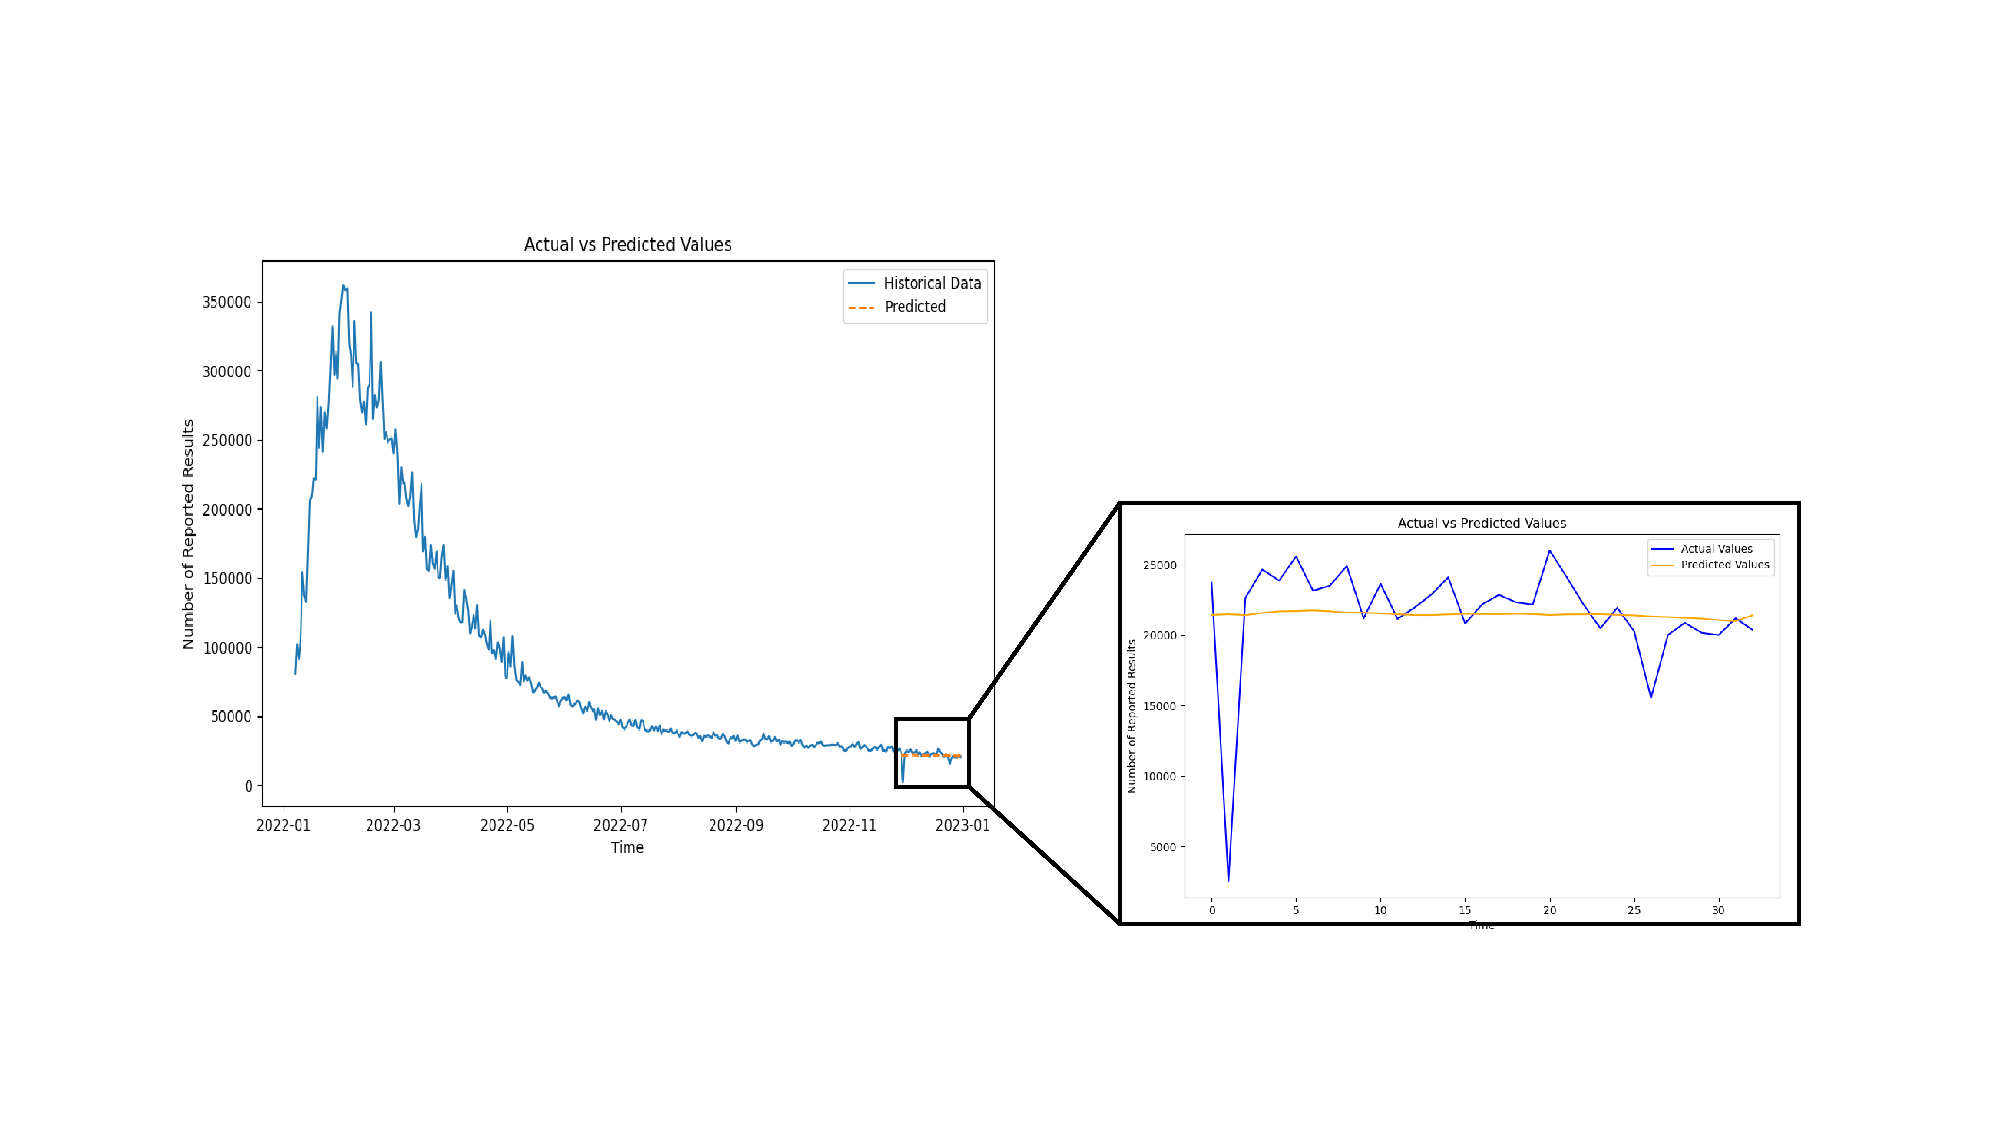
\includegraphics[width=18cm]{figure/F2.pdf}  % 引入图片源
        \caption{Actual vs Predicted Values} \label{Figure2}  % 标题与标签
\end{figure}  % 图片结束
We found that the results of this 
fitting had a good correlation with the actual values, so we also used the model to predict the next 90 days. 
The results are shown in Figure 3.
\begin{figure}[h]  % 图片
        \small
        \centering  % 居中
        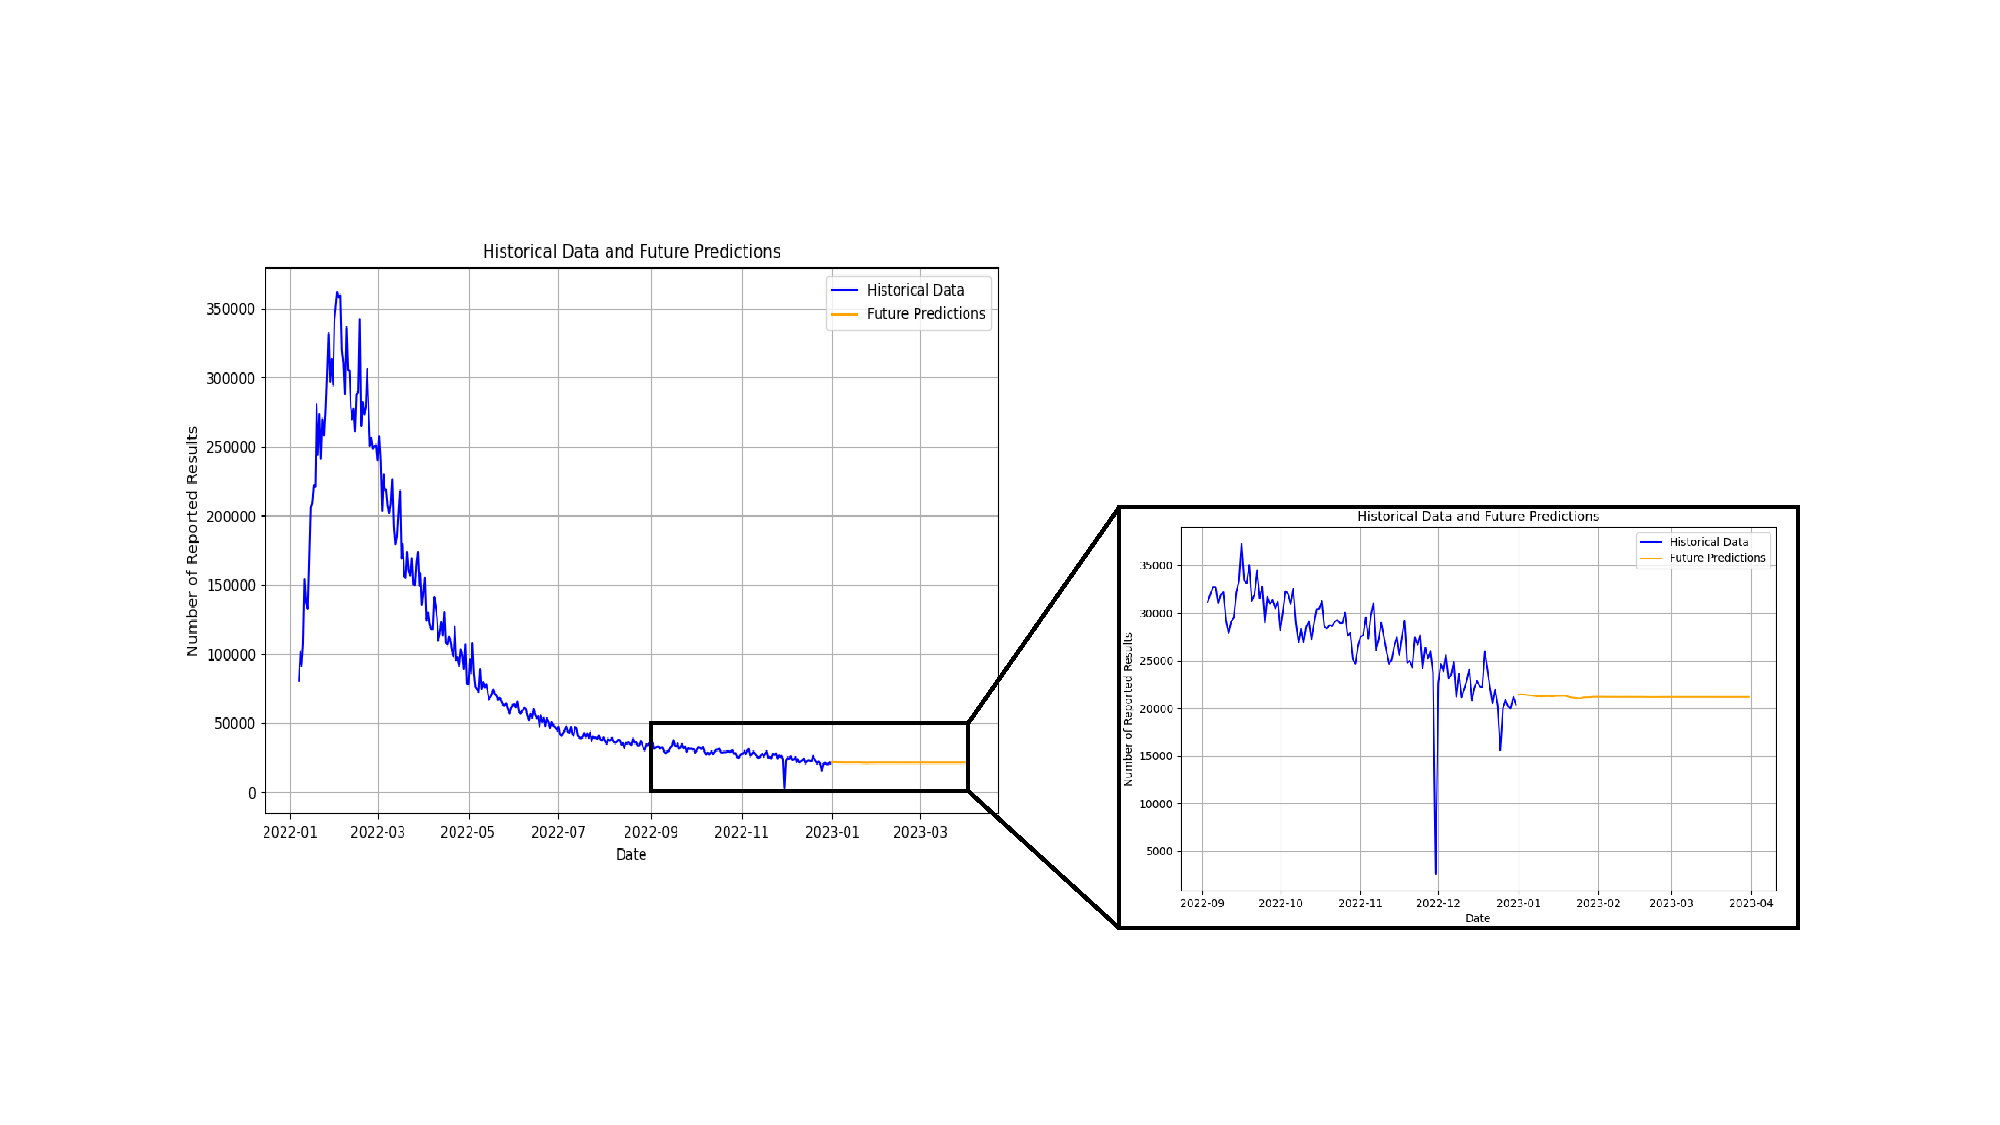
\includegraphics[width=18cm]{figure/F3.pdf}  % 引入图片源
        \caption{Historical Data and Future Predictions} \label{Figure2}  % 标题与标签
\end{figure}  % 图片结束


We also tracked the changes in training loss and validation loss over time. As the number of iterations increased, 
the training loss gradually decreased, indicating that our model was increasingly fitting the training data and 
learning the underlying patterns. Eventually, it stabilized around 2\% at the 10th iteration, suggesting that the 
model had converged and reached an optimal point. To prevent overfitting, we also closely monitored the changes 
in validation loss. Initially, we observed that the validation loss increased during the early iterations, likely 
due to the model adapting to the training data. However, after four iterations, it started to decrease, showing 
signs of generalization. By the 10th iteration, the validation loss had also stabilized, indicating that the model 
was no longer overfitting. We took the error value at the 10th iteration as the final result, and the data plot is 
shown in Figure 4, reflecting the training dynamics throughout the process.

\begin{figure}[h]  % 图片
        \small
        \centering  % 居中
        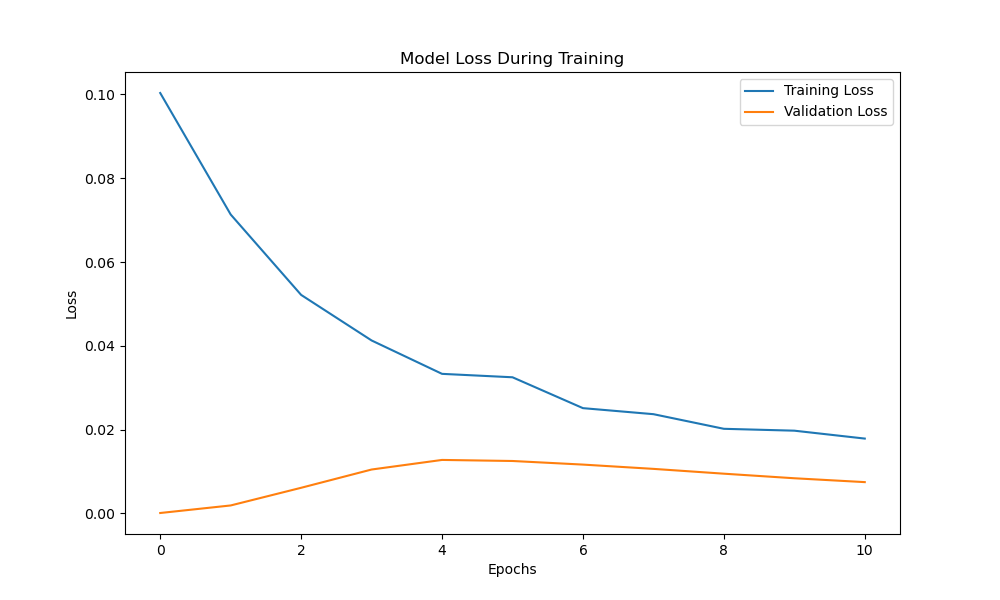
\includegraphics[width=14cm]{figure/F4.png}  % 引入图片源
        \caption{Model Loss During Training} \label{Figure4}  % 标题与标签
\end{figure}  % 图片结束

Based on our model, the predicted range for the number of reported results on March 1, 2023, is:
\begin{equation} 
        x_{March1,2023} =21137\pm 2.01425\%
\end{equation}  

\section{Relationship of Word Attributes and Scores from Percentage}

\subsection{Score setting}
The data provided in the problem is presented in percentages, which does not accurately reflect the actual scores for a given day. 
Therefore, we define the score for a specific day as follows:
\begin{equation}  
        score= w_{1}\ast \sum_{i=1}^{6} i\ast p_{i}+w_{2}\ast p_{x}
\end{equation}  
The score is determined by the number of correct guesses, meaning that 4 successful attempts would result in a score of 4. Since 
the game only has two possible outcomes, success or failure, we assign a weight of 0.5 to each outcome in order to balance the results.
\subsection{Frequency setting}

Considering that people from various industries are playing Wordle, we began to think about which types of words are more likely to be 
guessed. Since people from different industries have varying levels of expertise, their vocabulary also tends to differ, but the words 
they commonly use are generally those used in everyday life, such as "sleep," "lunch," and so on. Therefore, we believe that the frequency 
of a word's appearance will impact the results. To address this, we used google website\upcite{2} to collect statistics on the frequency of each word 
used in Wordle puzzles, denoted as $f_{word}$.
\subsection{Regression Analysis}
After defining frequency and score, we set them as the x-axis and y-axis, respectively, and plotted a scatter plot in Figure 5. Additionally, 
we created heatmaps in Figure 6 for frequency, score, and the number of attempts, and calculated the Pearson correlation to measure their correlation,
The formula is as follows:

\begin{equation}  % 公式,独占一行、居中,自动编号
        r=\frac{\sum (f_{word,i}-\bar{f_{word}})(score_{i}-\bar{score})}
        {\sqrt{\sum (f_{word,i}-\bar{f_{word} }})^2\sqrt{\sum (score_{i}-\bar{score}})^2} 
\end{equation}  % 公式结束

\begin{figure}[h]  % 图片
\centering  % 居中
\begin{minipage}[c]{0.48\textwidth}  % 子页
\centering  % 居中
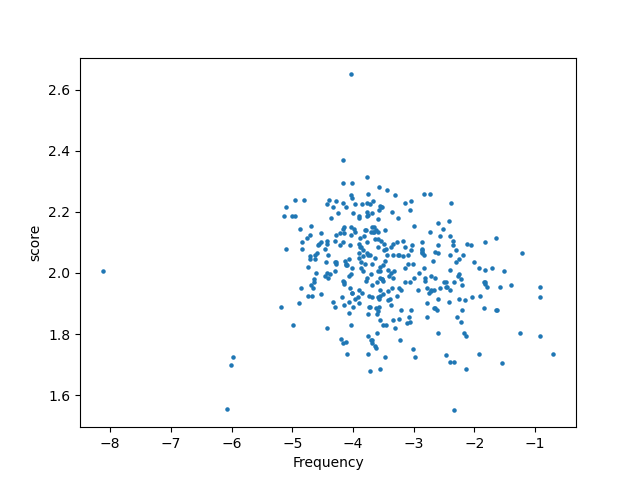
\includegraphics[width=7cm]{F5.png}  % 引入图片源
\caption{Word frequency} \label{Figure5}  % 标题与标签
\end{minipage}  % 子页结束
\hspace{0.02\textwidth}
\begin{minipage}[c]{0.48\textwidth}  % 子页
\centering  % 居中
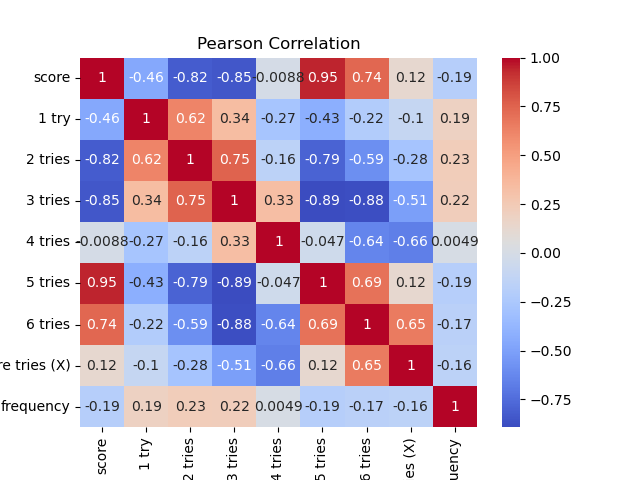
\includegraphics[width=7cm]{F6.png}  % 引入图片源
\caption{Pearson Correlation} \label{Figure6}  % 标题与标签
\end{minipage}  % 子页结束
\end{figure}  % 图片结束

From the plots, we observed that the correlation between a word's frequency and its score is only 0.19, indicating a weak correlation. 
We believe this is because, even though some words are frequently used in daily life, they may have synonyms that are more commonly used, 
causing the original words to be forgotten. For example, the word “mummy” from October 23, 2022. Additionally, some words have had their 
original meanings replaced by other associations. For instance, the word “watch” from March 11, 2022—due to the prevalence of smartphones, 
people now check the time on their phones rather than looking at a watch.Ultimately, we concluded that the frequency of a word's usage is u
nrelated to its performance in difficult modes.
\section{Model 2}  % 一级标题

\section{Model 3}  % 一级标题

\section{Interesting Findings}  % 一级标题
\subsection{4 Tries is the watershed}
What we are interested in is that through the heatmap of frequency and score, we found that 4 tries have almost no correlation with score 
and 5 tries, but there is a certain correlation with 3 tries.
Therefore, we believe this is because the majority of players are able to arrive at the correct answer within 3 to 4 attempts, which keeps 
4 tries in a dynamic balance. This makes 4 tries act as a constant in the statistical score, while a portion of players can only guess the 
correct answer in 5 tries or 6 tries. These two groups of players do not interfere with each other, which is why there is no correlation. 
We specifically plotted the correlation between 4 tries and 5 tries, and 3 tries for easier viewing. The detailed image is shown below.
\begin{figure}[h]  % 图片
        \centering  % 居中
        \begin{minipage}[c]{0.32\textwidth}  % 子页
        \centering  % 居中
        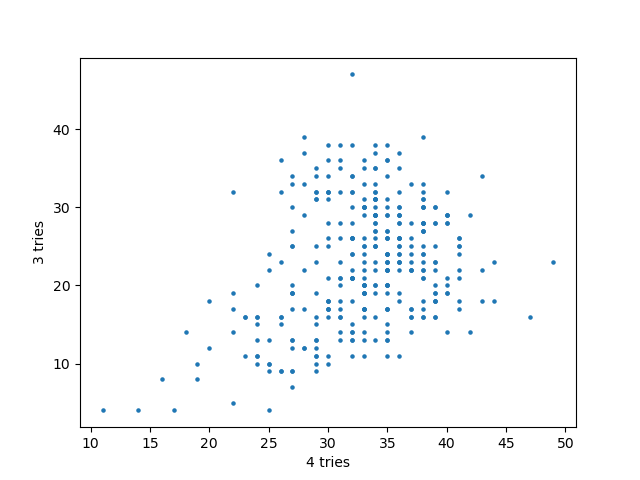
\includegraphics[width=5cm]{i2.png}  % 引入图片源
        \caption{4 and 3 tries'} \label{Figure9}  % 标题与标签
        \end{minipage}  % 子页结束
        \hspace{0.02\textwidth}
        \begin{minipage}[c]{0.32\textwidth}  % 子页
        \centering  % 居中
        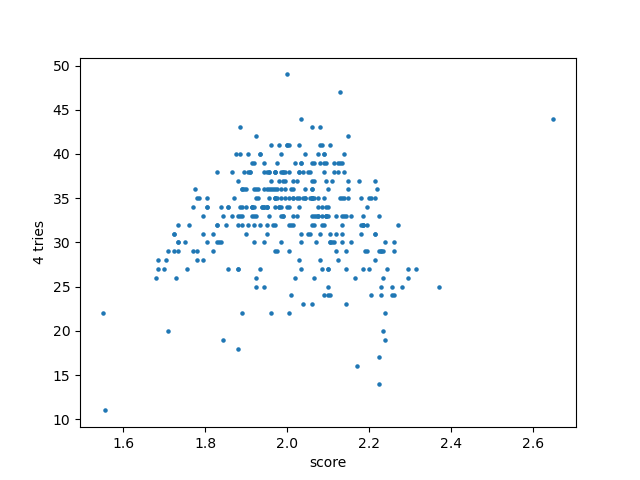
\includegraphics[width=5cm]{i1.png}  % 引入图片源
        \caption{4 tries and score's correlation} \label{Figure8}  % 标题与标签
        \end{minipage}  % 子页结束
        \begin{minipage}[c]{0.32\textwidth}
        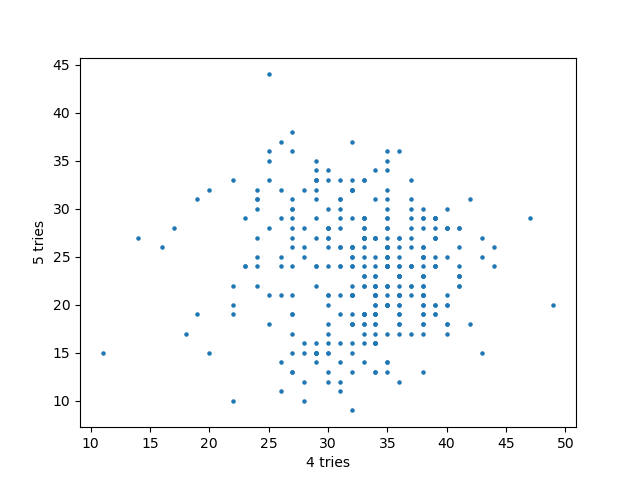
\includegraphics[width=5cm]{i3.png}  % 引入图片源
        \caption{4 and 5 tries'} \label{Figure10}  % 标题与标签
        \end{minipage}
\end{figure}  % 图片结束

\begin{figure}[h]  % 图片
        \small
        \centering  % 居中
        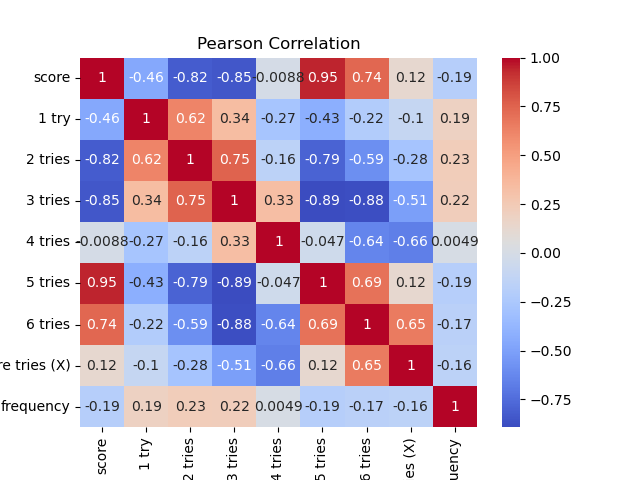
\includegraphics[width=14cm]{F6.png}  % 引入图片源
        \caption{Pearson Correlation} \label{Figure6}  % 标题与标签
\end{figure}  % 图片结束

\section{Sensitivety Analysis}  % 一级标题

\section{Model Assessment}

\subsection{Strengths}
\subsection{Weaknesses}

\section{Letter}
%\begin{figure}[h]  % 图片
%\small
%\centering  % 居中
%\includegraphics[width=12cm]{example.eps}  % 引入图片源
%\caption{example} \label{fig:example}  % 标题与标签
%\end{figure}  % 图片结束

% This is Figure \eqref{fig:example}.  % 引用图表

 \textit{I love math.}  % 斜体

\textbf{I love math.}  % 粗体

\underline{I love math.}  %下划线
%%%%%%%%%%%%%%%%%%%%%%%% 并排图 %%%%%%%%%%%%%%%%%%%%%%%%
%\begin{figure}[h]  % 图片
%\centering  % 居中
%\begin{minipage}[c]{0.48\textwidth}  % 子页
%\centering  % 居中
%\includegraphics[width=7cm]{example.eps}  % 引入图片源
%\caption{example} \label{fig:example}  % 标题与标签
%\end{minipage}  % 子页结束
%\hspace{0.02\textwidth}
%\begin{minipage}[c]{0.48\textwidth}  % 子页
%\centering  % 居中
%\includegraphics[width=7cm]{example.eps}  % 引入图片源
%\caption{example} \label{fig:example}  % 标题与标签
%\end{minipage}  % 子页结束
%\end{figure}  % 图片结束
%%%%%%%%%%%%%%%%%%%%%% 并排图结束 %%%%%%%%%%%%%%%%%%%%%%

\begin{thebibliography}{99}
        \bibitem{1} https://holidays-calendar.net/
        \bibitem{2} https://books.google.com/ngrams/
\end{thebibliography}

\printbibliography  % 打印引用文献列表

%%%%%%%%%%%%%%%%%%%%%%% 正文结束 %%%%%%%%%%%%%%%%%%%%%%%

\begin{appendices}  % 附录

\begin{memo}[Memorandum]  % 建议书
	This is a memorandum.
\end{memo}  % 建议书结束

\section{First appendix}  % 一级标题

Here are simulation programmes we used in our model as follow.\\
\textbf{MATLAB source code:}
%\lstinputlisting[language=Matlab]{./code/matlab.m}

\section{Second appendix}  % 一级标题

\textbf{Python source code:}
%\lstinputlisting[language=C++]{./code/python.py}

\end{appendices}  % 附录结束
\end{document}  % 文档结束
%%%%%%%%%%%%%%%%%%%%%%%%%%%%%%%%%%%%%%%%%%%%%%%%%%%%%%%   